\chapter{Introduzione}
\label{cha:intro}

Nel mondo in cui viviamo oggi la tecnologia ha raggiunto un livello di sviluppo senza precedenti. Nuovi smartphone, tablet e computer vengono presentati con al loro interno programmi per l'editing di immagini e video. La crescente disponibilità di questi dispositivi ha determinato un significativo aumento del volume di contenuti condivisi e questa tendenza non sembra fermarsi. Il grado di interconnessione raggiunto tra le persone permette loro di comunicare con maggiore facilità ma, allo stesso tempo, solleva numerose preoccupazioni dal punto di vista della sicurezza. Le informazioni condivise possono influenzare le idee e le azioni di molte persone. Come conseguenza, si pone il problema di garantire l'integrità e la veridicità dei media digitali. La diffusione di strumenti sempre più facili da utilizzare per la creazione di contenuti falsi forza lo sviluppo di contromisure. A supporto delle attività di controllo, il campo di ricerca della scienza multimediale forense, o \textit{media forensics}, ambisce ad identificare e contrastare manipolazioni e modifiche su immagini e video. Nelle sezioni seguenti verrà illustrata una breve panoramica sulle principali tematiche di ricerca che costituiscono la \textit{media forensics}, ponendo particolare attenzione al ruolo svolto dai social network.\\

\section{Social Media Forensics}
\label{sec:social_media_forensics}

Come riportato in~\cite{media_forensics_definition}, la \textit{media forensics} è definita come:

\begin{quote}
    \textit{“ lo studio scientifico sulla raccolta, l'analisi, l'interpretazione e la presentazione di prove audio, video e immagini ottenute nel corso di indagini e procedimenti giudiziari."}
\end{quote}
Il processo di digitalizzazione dei sistemi analogici, riferito a documenti audio, visivi e testuali, ha provocato un profondo cambiamento non solo in ambito lavorativo ma anche nella vita quotidiana~\cite{digitalizzazione}. In questo contesto, la \textit{media forensics} ha assunto un'importanza sempre più rilevante. Tuttavia, l'immenso numero di azioni che possono essere svolte sugli oggetti digitali e gli innumerevoli campi di applicazione di questa disciplina non facilita il lavoro dei ricercatori. L'analisi delle manipolazioni effettuate sui contenuti digitali, l'identificazione della camera di acquisizione attraverso univoche impronte digitali e lo sviluppo di nuove tecniche per verificare la reale origine di immagini e video sono solo alcuni esempi.\\
Ogni giorno miliardi di contenuti vengono caricati dagli utenti tramite social media, applicazioni di messaggistica, blog, forum e piattaforme di streaming. Stando a quanto riportato dagli ultimi studi~\cite{chaffey}, nel 2022 più del 58\% della popolazione mondiale (circa 4,68 miliardi di persone) utilizza almeno un social media (es., YouTube, Facebook, Instagram) e servizi come WhatsApp e Telegram. Negli ultimi 12 mesi, 424 milioni di nuovi utenti  si sono registrati su queste piattaforme. La crescente popolarità (Fig.~\ref{fig:social_networks}) e la facile accessibilità ai social network ha permesso agli utenti di condividere ogni aspetto della loro vita, esponendosi pubblicamente ed eliminando ogni forma di barriera spazio-temporale. Non sempre, però, vengono utilizzate in modo consapevole, sottovalutando alcuni aspetti che possono rivelarsi pericolosi. È proprio in questo contesto che trovano spazio una serie di azioni illecite messe in atto da malintenzionati che generano e diffondono contenuti digitali falsi. La manipolazione di immagini e video non è uno strumento legato unicamente alla sfera del singolo individuo, bensì un preoccupante fenomeno di massa. Di conseguenza, vi è il rischio di non riuscire più a determinare ciò che è vero. La necessità di sviluppare metodi e tecniche per la salvaguardia dei contenuti multimediali assume quindi un ruolo chiave~\cite{pagano}.

\begin{figure}[h!]
    \centering
    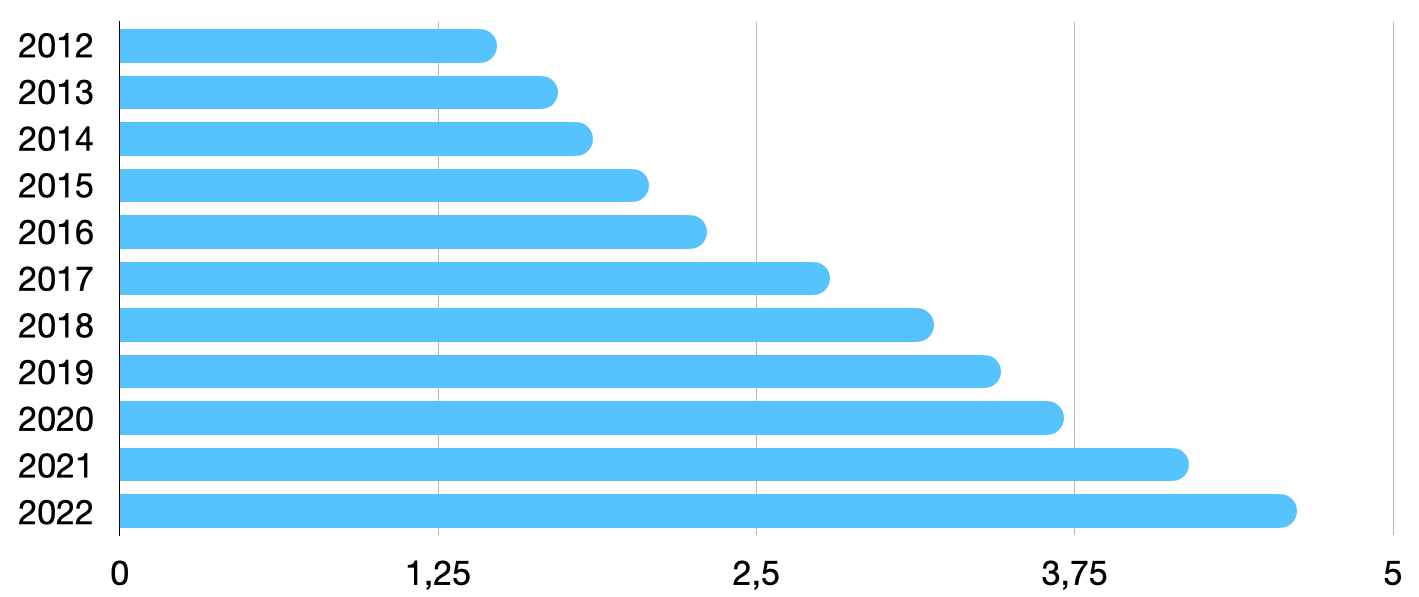
\includegraphics[width=15cm,height=12cm,keepaspectratio]{Immagini/statistiche_social.png}
    \caption{Istogramma a colonne che mostra il numero totale (in miliardi) di utenti utilizzatori di social media a partire da gennaio 2012~\cite{kemp}.}
    \label{fig:social_networks}
\end{figure}

\noindent
L'origine della \textit{social media forensics} è strettamente legata allo sviluppo e alla diffusione dei social network. Fino a poco tempo fa, la maggior parte degli studi condotti in questo ambito è stata eseguita in condizioni controllate e avendo a disposizione informazioni pregresse sul problema analizzato. Solo di recente i ricercatori hanno provato ad estendere questo campo in scenari di vita reale. I risultati ottenuti sono duplici: da un lato si migliora la comprensione del percorso svolto in rete da un oggetto digitale, permettendo di identificare fake news e verificare l'integrità delle informazioni; dall'altro si presentano nuove sfide derivanti dalla possibilità da parte degli utenti di caricare o condividere (anche molteplici volte) immagini e video, comportando un progressivo deterioramento del dato multimediale.\\
Il ciclo di vita di un contenuto digitale è caratterizzato da molteplici fasi~\cite{pasquini2021media}. Ogni step di questo processo lascia tracce distintive che possono essere identificate tramite tecniche differenti. La \textit{social media forensics}, pertanto, può essere suddivisa in tre macro-campi di applicazione: la \textit{forensics analysis}, la \textit{platform provenance analysis} e la \textit{multimodal verification analysis}. Ognuno di questi rami della ricerca risponde a quesiti ben specifici:

\begin{itemize}
    \item \textit{“Quali sono le operazioni compiute su immagini e video durante le fasi di acquisizione e post-processing? Da quale dispositivo provengono?"}
    \item \textit{“Quali sono i social network utilizzati per il caricamento dei contenuti?"}
    \item \textit{“Gli elementi analizzati sono veri oppure falsi? Sono stati inseriti in un contesto sbagliato?"}
\end{itemize}

\subsection{Forensics analysis}
\label{sub_sec:forensics_analysis}

La \textit{forensics analysis} analizza i contenuti digitali per individuare potenziali manomissioni e/o modifiche che minano la credibilità delle informazioni~\cite{bartolucci}. Possiamo riassumere gli obiettivi di questa disciplina in due punti:

\begin{itemize}
    \item Risalire alla fotocamera o al sensore che ha acquisito un determinato oggetto digitale (\textit{source identification});
    \item Verificare che questo oggetto non sia stato alterato tramite operazioni non autorizzate (\textit{integrity verification}).
\end{itemize}

\subsubsection{Source identification}
\label{sub_sub_sec:source_identification}

Con il termine \textit{source identification} ci si riferisce al processo di tracciamento del dispositivo che ha prodotto un particolare contenuto digitale (es., immagine o video). In questo campo i ricercatori hanno analizzato immagini e video con l'obiettivo di trovare risposte a questioni ancora aperte. Nel caso delle immagini sono stati condotti un numero maggiore di lavori data l'ampia disponibilità di dati e la minore complessità del problema. Gestire i video, infatti, è più complicato per via delle dimensioni dei file. I metodi proposti, come spiegato in~\cite{verdoliva}, possono essere suddivisi in due principali categorie: hardware e software. L'approccio hardware studia gli effetti generati dalle lenti o difetti presenti nel sensore durante l'acquisizione, quello software, invece, considera le operazioni di elaborazione compiute dalla camera.\\
Con la nascita dei social network i metodi classici di analisi (es., copy-paste, splicing) sono diventati obsoleti. Le cause principali sono da ricercarsi nelle differenti policy adottate da queste piattaforme. Come risultato, le modifiche apportate nei media digitali dai processi di condivisione e upload/download causano un deterioramento se non una completa cancellazione delle informazioni lasciate dal dispositivo di acquisizione. Gli studi più recenti propongono tecniche basate sul PRNU  (\textit{Photo Response Non-Uniformity})~\cite{bertini2015profile}, sui video file containers~\cite{lopez2020digital} e le \textit{convolutional neural networks}~\cite{rafi2019application}.


\subsubsection{Integrity verification}
\label{sub_sub_sec:integrity_verification}

Se per la \textit{source identification} sono state condotte svariate indagini, lo stesso non si può dire per l'\textit{integrity verification} che per quanto riguarda lo studio di dati provenienti da social network risulta un ramo della disciplina abbastanza inesplorato. Con \textit{integrity verification} si definisce il processo finalizzato alla verifica dell'integrità delle informazioni, tramite l'individuazione di alterazioni causate dall'esecuzione di particolari operazioni.\\
Nell'ambito della \textit{social media forensics}, questa definizione viene applicata ai contenuti digitali che sono stati condivisi tramite diverse piattaforme social e il cui obiettivo è assicurarne la correttezza. Tuttavia, queste verifiche vengono ampiamente ostacolate dalle operazioni compiute da siti web e applicazioni, che possono causare la cancellazione degli indizi su eventuali anomalie. Le poche ricerche condotte in questo ambito hanno impiegato le stesse tecniche utilizzate per le \textit{source identification}. Nel prossimo futuro, lo sviluppo di nuovi metodi potrà offrire ulteriori spunti per la ricerca.


\subsection{Platform provenance analysis}
\label{sub_sec:platform_provenance_analysis}

I social network hanno radicalmente cambiato il mondo, offrendo possibilità che precedentemente non erano nemmeno immaginabili. Se da un lato permettono l'immediata comunicazione tra le persone, dall'altro si contrappongono rischi significativi legati alla sicurezza. Basti pensare al caso in cui, durante un processo, si ha la necessità di individuare l'origine di un file, per risalire all'identità della persona che lo ha diffuso.\\
Il ramo di ricerca della \textit{platform provenance analysis} ha come principale obiettivo quello di ricostruire la storia associata ad un contenuto digitale. È possibile identificare alcuni punti chiave che stanno alla base di questa disciplina:

\begin{itemize}
    \item Risalire alle piattaforme che hanno processato l'oggetto digitale;
    \item Ricostruire l'intera storia di condivisione dell'oggetto digitale;
    \item Estrarre informazioni significative sui sistemi utilizzati nella fase di upload.
\end{itemize}
Per raggiungere tali obiettivi si può analizzare il problema utilizzando metodi di classificazione in cui immagini e video vengono raggruppati basandosi sulla cronologia passata delle condivisioni.\\
Il processo risolutivo (Fig.~\ref{fig:plat_prov_analy}) è il risultato di una serie di fasi sequenziali che prevede come prima operazione l'adozione di un dataset (raccolta di immagini e/o video) che definisca in maniera esaustiva lo scenario affrontato. Possono essere impiegati dataset proprietari generati da zero oppure quelli resi pubblicamente accessibili dalla comunità scientifica. Tra i più importanti troviamo: RAISE~\cite{dang2015raise}, VISION~\cite{shullani2017vision} e UCID~\cite{schaefer2003ucid}.\\
A questo punto, partendo dalle immagini/video presenti nel dataset vengono estratte informazioni rilevanti, o \textit{feature}. Il numero di operazioni che possiamo svolgere su questi dati sono molteplici e distinguibili in due grandi categorie: nella prima troviamo quelle che si concentrano sull'analisi del segnale dell'immagine, mentre nella seconda quelle operazioni che considerano i metadati. Se da un lato l'analisi del segnale permette di ottenere informazioni attraverso lo studio dei pixel per costituire \textit{feature} di tipo statistico (es., istogrammi dei coefficienti DCT), dall'altro i metadati consentono di ricavare in maniera rapida informazioni secondarie (es., tempo e dispositivo di acquisizione e coordinate GPS). Vari approcci includono l'utilizzo combinato dei due sistemi di analisi.\\
La classificazione finale è eseguita tramite l'impiego di algoritmi di \textit{machine learning} adeguatamente allenati con le \textit{feature} estratte nella fase precedente. Gli approcci proposti sono molteplici: si passa dai classici metodi di classificazione supervisionata (es., \textit{support vector machine} o \textit{random forest}) fino ad adottare tecniche di \textit{deep learning}.

\begin{figure}[h!]
    \centering
    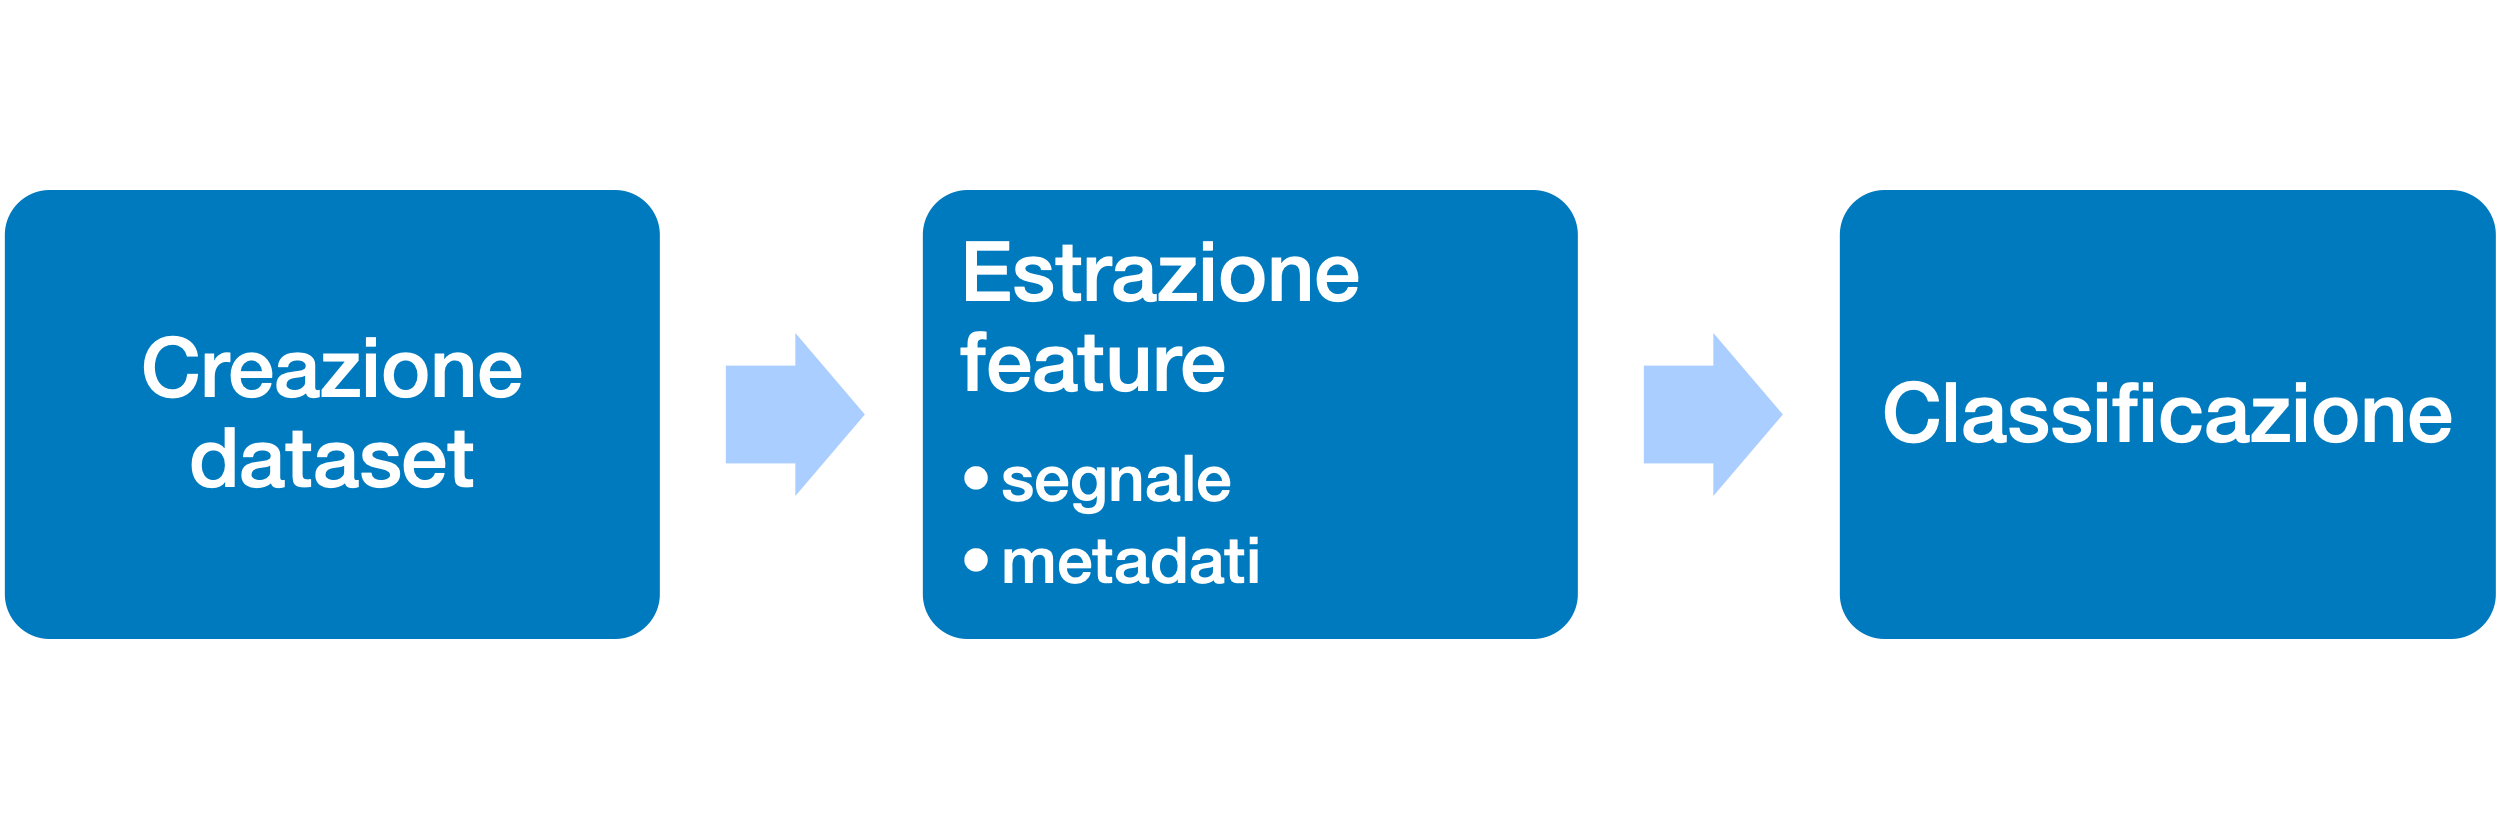
\includegraphics[width=12cm,height=9cm,keepaspectratio]{Immagini/platform_provenance_analysis.png}
    \caption{Processo seguito per la \textit{platform provenance analysis}.}
    \label{fig:plat_prov_analy}
\end{figure}

\subsection{Multimodal verification analysis}
\label{sub_sec:multimodal_verification_analysis}

La costante crescita di popolarità delle piattaforme digitali ha determinato un cambiamento del modo in cui le persone ricercano e ricevono informazioni. Se fino a non molto tempo fa telegiornali, riviste e notiziari erano la principale fonte di comunicazione, adesso lo scenario è cambiato: annunci e notizie dal mondo vengono raccolte e diffuse da blog, forum e applicazioni proprietarie. La velocità di diffusione delle informazioni ha eliminato ogni confine ma, al tempo stesso, la possibilità che vengano manipolate o addirittura create ad hoc rappresenta uno scenario preoccupante. Campagne politiche, fake news, attacchi terroristici, teorie cospirazioniste, come anche notizie vere ma decontestualizzate, necessitano di sistemi di regolazione.\\
Il ramo di ricerca della \textit{multimodal verification analysis} studia i metodi utilizzati per diffondere disinformazione con due principali scopi: scovare eventuali modifiche delle informazioni diffuse e identificare qualora una notizia vera sia stata volutamente associata all'interno di un contesto sbagliato. Così come avviene nella \textit{platform provenance analysis}, anche la \textit{multimodal verification analysis} dedica particolare attenzione all'analisi delle operazioni veicolate tramite i social network. Le condivisioni sulle diverse piattaforme (es., Twitter, Instagram, Facebook) hanno strutture differenti in base al tipo di post utilizzato: solo testo, immagini/video oppure una combinazione dei due.\\
L'analisi prende in considerazione tre tipologie di elementi:

\begin{itemize}
    \item Informazioni visive ricavate da immagini o video associati agli oggetti digitali condivisi;
    \item Informazioni testuali derivate dal testo associato ai post pubblicati;
    \item Metadati ricavati dalla combinazione di due fattori: quelli strettamente legati al contenuto digitale condiviso e quelli che prendono in considerazione l'utente che ha diffuso le informazioni (es., numero di commenti, numero di follower, frequenza di pubblicazione, etc.)
\end{itemize}
In conclusione, il dominio di applicazione della \textit{social media forensics} è rappresentato dalla \textit{forensics analysis}, dalla \textit{platform provenance analysis} e dalla \textit{multimodal verification analysis} (Fig.~\ref{fig:mappa}). I metodi e le soluzioni fornite da queste discipline non sono unicamente ristretti alla pura ricerca, ma possono offrire un contributo attivo nella fase di investigazione.

\section{Obiettivi}
\label{sec:obiettivi}

Il lavoro proposto in questa tesi rientra nell'ambito della \textit{platform provenance analysis}, ma propone un aspetto nuovo e fino ad ora inesplorato. La maggior parte dei lavori svolti in questo campo tende a considerare molteplici piattaforme di condivisione, cercando di ricostruire la catena di social in cui un contenuto digitale è stato diffuso. Nel nostro caso, invece, consideriamo un solo social network, WhatsApp, ma cerchiamo di risalire al tipo di device e al sistema operativo utilizzato per l'upload. Nei prossimi capitoli forniremo un'analisi dei lavori più rilevanti svolti nel campo della \textit{platform provenance analysis}, dopodiché mostreremo l'approccio da noi adottato e i risultati finali ottenuti.

\begin{figure}[h!]
    \centering
    \adjustbox{scale=0.45}{
    \begin{tikzpicture}[
        mindmap,
        grow cyclic, text width=4cm, align=flush center,
        every node/.style={concept, font=\fontsize{6mm}{6mm}\selectfont},
        concept color=orange!40,
        level 1/.style={level distance=9.2cm, sibling angle=120},
        level 2/.style={level distance=6.2cm, sibling angle=60}
    ]
    
    \node [root concept, scale=2] {\textbf{Social media forensics}}
        child [concept color=blue!30] {node {\textbf{Forensics analysis}}
            child {node {Identificazione sorgente}}
            child {node {Verifica integrità}}
        }
        child [concept color=teal!40] {node {\textbf{Platform provenance analysis}}
            child {node {Identificazione piattaforme di condivisione}}
            child {node {Ricostruzione storia oggetto digitale}}
            child {node {Estrazione informazioni dai sistemi di upload}}
        }
        child [concept color=yellow!30] {node {\textbf{Multimodal verification analysis}}
            child {node {Verifica credibilità dei contenuti}}
            child {node {Identificazione informazioni false}}
            child {node {Individuazione dati sintetici}}
        };
    \end{tikzpicture}
    }
    \caption{Le tre macro-categorie che compongono la \textit{social media forensics}.}
    \label{fig:mappa}
\end{figure}


